\documentclass[11pt, a4paper, twocolumn]{article}

\usepackage{style} 


% Information for generating title
\title{\bfseries Machine Learning: Project 1}
\author{\textbf{Olivier Stähli} \\ \href{mailto:olivier.staehli@epfl.ch}{olivier.staehli@epfl.ch}
   \and \textbf{Ivan Bioli} \\ \href{mailto:ivan.bioli@epfl.ch}{ivan.bioli@epfl.ch}
   \and \textbf{Fabio Matti} \\ \href{mailto:fabio.matti@epfl.ch}{fabio.matti@epfl.ch}}
\date{}

\begin{document}

% Escaping twocolumn-layout to generate titlelines and abstract
\twocolumn[
  \begin{@twocolumnfalse}
    \vspace{-1.5cm}
    \maketitle
    \vspace{-1cm}
    \begin{abstract}
        We implement six standard regressors. Subsequently, the Higgs boson data set for binary classification from 30 numerical features is used for testing our implementations. We perform various preprocessing techniques and tune the parameters of our regressors to maximize accuracy, as first priority, and F1-score of the predictions, as second priority. Additionally, an optimized regressor for this specific task is developed.
    \end{abstract}
    \vspace{0.75cm}
  \end{@twocolumnfalse}
]

\section{Introduction}
\label{sec:introduction}

The features in the data set refer to numerical measurements coinciding with the observation of a decay signature, either caused by an event involving a Higgs boson ('s' for signal) or  not related to Higgs bosons ('b' for background) \cite{higgs2014}. Based on 250'000 training samples, our goal is to predict the unknown labels for the test data.

\section{Models and Methods}
\label{sec:models}

\subsection{Preprocessing}
\label{subsec:preprocessing}
In a first step, we visualized and analyzed the data. We modified the features that showed undefined values, which were set by default to -999 \cite{higgs2014}. We tried replacing these undefined values with zero, the mean value or the median value of the feature (computed ignoring the undefined values). Among these approaches, the latter proved to be the most effective solution. We also tried adding a binary variable indicating that the corresponding entry of the feature was undefined, which did not prove to be effective.

Subsequently, we replaced outliers, i.e. values that deviate  from the mean value more than three times the standard deviation according to the Grubbs' definition \cite{Grubbs69}, by the mean value of the feature. 

The feature  \enquote{PRI\_jet\_num}  is a discrete variable. Therefore, for the standard regressors, we tried adding a binary feature for each number of jets. However, this approach did not lead to any improvement in accuracy.  Our optimized regressor exploits the \enquote{PRI\_jet\_num} feature to train a model for each number of jets. For a more detailed description of our approach, see \Cref{subsubsec:optimized regressor}.

As a final preprocessing step, we augmented the features using a polynomial basis of degree $D$ with or without offset, and standardized the features by subtracting the mean value and dividing by the standard deviation.

The improvements to which our preprocessing leads are shown in \Cref{fig:preprocessing}.
\begin{figure}[htp]
    \centering
    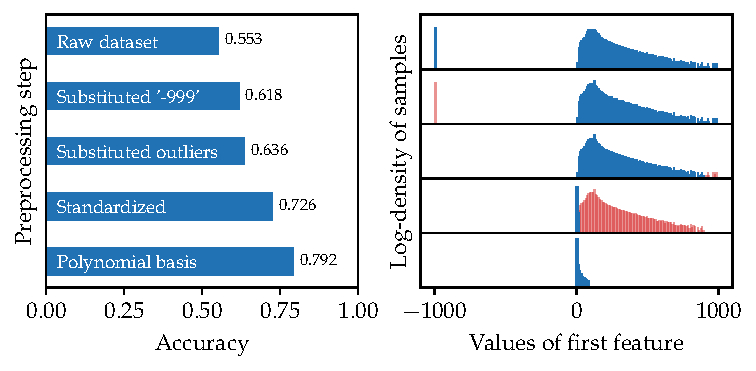
\includegraphics[width=\columnwidth]{figures/preprocessing.pdf}
    \caption{On the right, the effect every preprocessing step has on the distribution of the values (here for the first feature). On the left, the progression of the mean accuracy in a 4-fold cross validation on the training set with regularized logistic regression.}
    \label{fig:preprocessing}
\end{figure}

\vspace{-8pt}
\subsection{Implementations}
\label{subsec:implementations}

We implemented the six proposed regressors in Python, based on their description
in \cite{jaggi2021}. Our implementations solely rely on the NumPy 1.21.1 library.
The source code is available on our \href{https://github.com/CS-433/ml-project-1-thelearningwolves.git}{Git repository}.

We paid particular attention to the following aspects:
\begin{itemize}
    \vspace{-8pt}
    \item Robustness: We implemented the regressors so that they can process any NumPy ndarray object as data matrix by diligent reshaping of arrays. Furthermore, we included \enquote{exp-guards} that prevent exponential functions from overflowing.
    \vspace{-8pt}
    \item Simple minimal working example: Each of our regressors may be fitted by just processing the training data without any other parameters.
\end{itemize}

\vspace{-8pt}
\subsubsection{Optimized regressor}
\label{subsubsec:optimized regressor}
The detailed description of the features in the dataset documentation \cite{higgs2014}, highlights that some features are systematically undefined for some values of the \enquote{PRI\_jet\_num} feature. For our optimized regressor, we therefore split our training set according to the four different jet numbers and trained four separate models. After splitting, the following operations were separately performed  on each of the reduced training sets. Constant columns in the reduced sets, like \enquote{PRI\_jet\_num} and those with only undefined values, were removed. The preprocessing was then carried out in the same way as described in \Cref{subsec:preprocessing}. To train the four separate models, we used as a base regressor one of the regressors proposed in the project description. Finally, we generated predictions for each number of jets separately.

\subsection{Parameter tuning}
\label{subsec:tuning}

We tuned our regressors through a 4-fold cross validation on the training set. Since we were dealing with a classification problem, instead of using a loss function, we used the accuracy as an indicator of how good our predictions are. The achieved accuracy is visualized through a grid-plot (see \Cref{fig:paramter_grid_search}). This type of visualization allows us extracting suitable parameters for our regressors. It also serves as an indicator of how stable the parameters are. If next to our ideal parameter, the accuracy falls off immediately, we avoid choosing this one, because of the uncertainty of whether this parameter will fail on the test set or not.

\begin{figure}[htp]
    \centering
    \begin{subfigure}[b]{0.49\columnwidth}
         \centering
         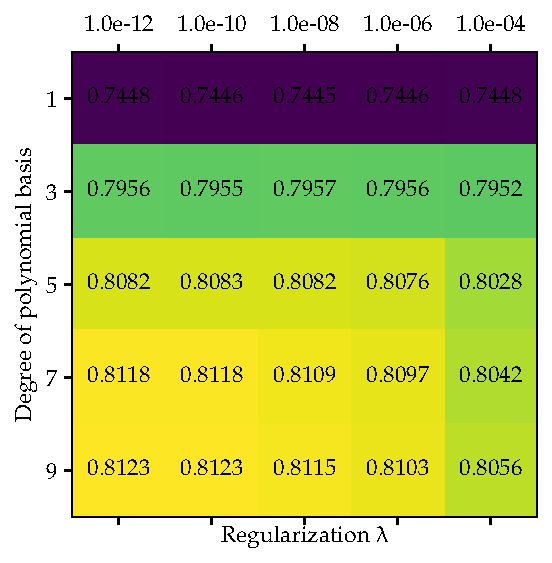
\includegraphics[width=\textwidth]{figures/ridge_regression_gridsearch_coarse.pdf}
         \caption{Coarse grid search.}
     \end{subfigure}
     \hfill
     \begin{subfigure}[b]{0.49\columnwidth}
         \centering
         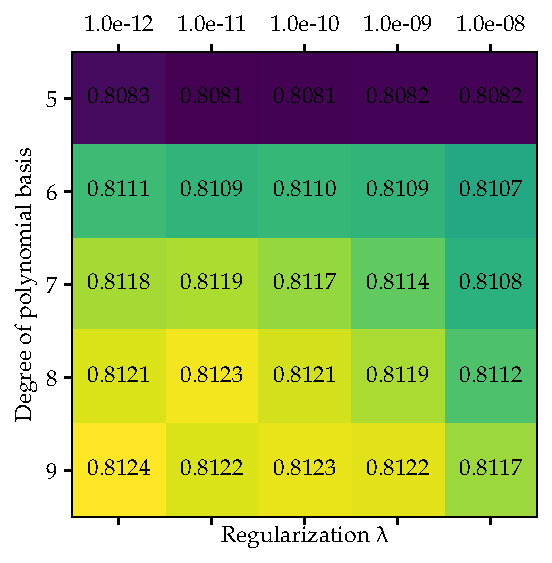
\includegraphics[width=\textwidth]{figures/ridge_regression_gridsearch_finer.pdf}
         \caption{Finer grid search.}
     \end{subfigure}
    \caption{Visualization used for tuning the parameters. Here, the ridge regressor was used in a 4-fold cross-validation. The accuracy is plotted on a grid for various choices of the regularization parameter $\lambda$ and the degree of the polynomial basis. Once a coarse grid search is done, a finer grid search is performed to find the parameters.}
    \label{fig:paramter_grid_search}
\end{figure}

The best set of parameters for each regressor can be found in Table \ref{tab:params}.

\begin{table}[ht]
    \caption{Ideal parameters for the regressors found by means of grid-search and 4-fold cross-validation. $D$ is the degree of the polynomial basis, $\lambda$ is the regularization parameter, $N$ is the maximum number of iterations, and $\gamma$ is the learning rate. If used, the initial parameter vector $\boldsymbol{w}_0$ was always set to zero.}
    \label{tab:params}
    \small
    \centering
    \renewcommand{\arraystretch}{1.1}
    \begin{tabular}{@{}lcccc@{}}
        \toprule
        Regressor & $D$ & $\lambda$ & $N$ & $\gamma$ \\
        \midrule
        least\_squares\_GD & 4 & - & 200 & 0.07 \\
        least\_squares\_SGD & 4 & - & 1e+5 & 5e-4 \\
        least\_squares & 8 & - & - & -  \\
        ridge\_regression & 8 & 1e-11 & - & - \\
        logistic\_regression & 4 & - & 500 & 2e-6 \\
        reg\_logistic\_regression & 4 & 1e-4 & 500 & 2.5e-6 \\
        optimized\_ridge & 9 & 1e-13 & - & - \\
        optimized\_logistic & 5 & - & 500 & 1e-5 \\
        optimized\_reg\_logistic & 8 & 1e-9 & 500 & 6.3e-6 \\
        \bottomrule
    \end{tabular}
\end{table}

\section{Results}
\label{sec:results}
The F1-score and accuracy our regressors were able to achieve are provided in \Cref{tab:results}. For our optimized regressor, as a base regressor we use the best linear regressor, i.e. ridge regression, and both logistic regressors.

% TODO: Links to submissions
\begin{table}[ht]
    \caption{Prediction performances achieved with the regressors on 
             the parameters specified in \ref{tab:params}. The regressor's
             names are clickable links to the respective submission.}
    \label{tab:results}
    \centering
    \small
    \renewcommand{\arraystretch}{1.1}
    \begin{tabular}{@{}lcc@{}}
        \toprule
        Regressor & F1-score & Accuracy \\
        \midrule
        \href{https://www.aicrowd.com/challenges/epfl-machine-learning-higgs/submissions/164066}{least\_squares\_GD} & 0.666 & 0.789 \\
        \href{https://www.aicrowd.com/challenges/epfl-machine-learning-higgs/submissions/164068}{least\_squares\_SGD} & 0.626  & 0.773\\
        \href{https://www.aicrowd.com/challenges/epfl-machine-learning-higgs/submissions/164069}{least\_squares} & 0.711 & 0.814 \\
        \href{https://www.aicrowd.com/challenges/epfl-machine-learning-higgs/submissions/163533}{ridge\_regression} & 0.711 & 0.814 \\
        \href{https://www.aicrowd.com/challenges/epfl-machine-learning-higgs/submissions/163297}{logistic\_regression} & 0.679 & 0.805 \\
        \href{https://www.aicrowd.com/challenges/epfl-machine-learning-higgs/submissions/163299}{reg\_logistic\_regression} & 0.699 & 0.806 \\
        \href{https://www.aicrowd.com/challenges/epfl-machine-learning-higgs/submissions/164216}{optimized\_ridge} & 0.731 & 0.826 \\
        \href{https://www.aicrowd.com/challenges/epfl-machine-learning-higgs/submissions/163557}{optimized\_logistic} & 0.711 & 0.812\\
        \href{https://www.aicrowd.com/challenges/epfl-machine-learning-higgs/submissions/163862}{optimized\_reg\_logistic} & 0.718 & 0.817 \\
        \bottomrule
    \end{tabular}
\end{table}

\section{Discussion}
\label{sec:discussion}
Following the discussion in \cite{jaggi2021}, we expected linear models not to be particularly suitable to classification problems, such as the present one. However, among the proposed regressors, the ridge regressor reaches a higher accuracy with respect to the logistic and the regularized logistic regressors. This might be due to the fact that the dataset is not too unbalanced and we remove extreme values through preprocessing. Furthermore, our optimized regressor improved the accuracy and the F1-score by more than 1\% and, once again, the adoption of the ridge regressor as a base regressor leads to better results with respect to the use of logistic regressors. 

\newpage
\nocite{*}
\printbibliography

\end{document}
